\section{Inner loop integration} \label{sec:inner_loop_integration}

The projected gradient descent architecture established in Algorithm~\ref{alg:inexact_pgd} relies on the Euclidean projection operator $\mathcal{P}_{\mathcal{H}}(\cdot)$ to enforce the physical monotonicity of the KR map. Evaluating this projection requires computing an infinite sequence of Dykstra iterations. In a practical software implementation, the inner loop must be truncated. However, applying a static iteration ceiling to the Dykstra algorithm throughout the entire training process introduces computational inefficiencies. To scale the framework to higher-dimensional tensor bases and larger particle sets, we implement a highly optimised, inexact projection solver.

\subsection{Dynamic iteration scheduling}
During the early stages of the outer learning loop (when $t$ is small), the unconstrained iterate $w^\circ$ is far from the optimal map parameterisation, and the gradient descent step size $\eta^{(t)}$ is large. Computing a high-precision projection at this stage wastes computational resources, as the subsequent unconstrained step will immediately displace the coefficients by a large margin. Conversely, as $t$ approaches the maximum outer iteration budget $T-1$ and the optimiser settles into a narrow minimum, high-precision projections become necessary to guarantee the final map is a valid diffeomorphism.

To balance precision and computational cost, we dynamically scale the inner Dykstra iteration budget based on the outer learning iteration $t$. We define a base iteration limit $M_{\mathrm{base}} \in \mathbb{N}$ and an inexact growth exponent $p \ge 1$. At outer iteration $t$, the maximum number of full Dykstra cycles (where one cycle consists of $n$ individual half-space projections) is given by the schedule:
\begin{equation}
    M^{(t)} = \lfloor M_{\mathrm{base}} (t+1)^p \rfloor.
    \label{eq:dynamic_budget}
\end{equation}
The dynamic iteration profile is visualised in Figure~\ref{fig:dynamic_iteration_budget}. This polynomial growth schedule ensures that the early gradient steps rely on cheap, approximate projections, while the later iterations enforce feasibility more aggressively.

\begin{figure}[htpb]
    \centering
    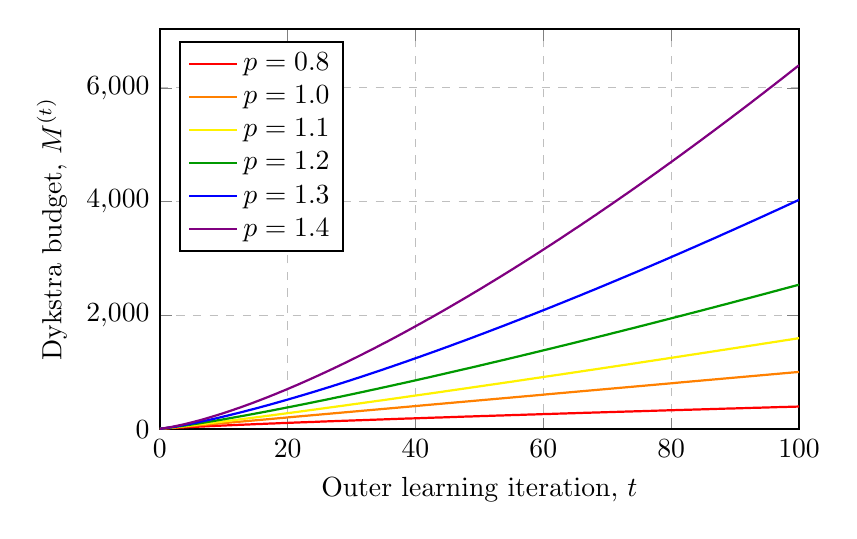
\begin{tikzpicture}
        \begin{axis}[
            width=0.8\textwidth,
            height=0.55\textwidth,
            xlabel={Outer learning iteration, $t$},
            ylabel={Dykstra budget, $M^{(t)}$},
            xmin=0, xmax=100,
            ymin=0,
            grid=major,
            grid style={dashed, gray!50},
            legend pos=north west,
            legend cell align={left},
            thick
        ]

        \addplot[domain=0:100, samples=200, color=red] {floor(10*(x+1)^0.8)};
        \addlegendentry{$p = 0.8$}
        
        \addplot[domain=0:100, samples=200, color=orange] {floor(10*(x+1)^1.0)};
        \addlegendentry{$p = 1.0$}
        
        \addplot[domain=0:100, samples=200, color=yellow] {floor(10*(x+1)^1.1)};
        \addlegendentry{$p = 1.1$}
        
        \addplot[domain=0:100, samples=200, color=green!60!black] {floor(10*(x+1)^1.2)};
        \addlegendentry{$p = 1.2$}
        
        \addplot[domain=0:100, samples=200, color=blue] {floor(10*(x+1)^1.3)};
        \addlegendentry{$p = 1.3$}
        
        \addplot[domain=0:100, samples=200, color=violet] {floor(10*(x+1)^1.4)};
        \addlegendentry{$p = 1.4$}
        
        \end{axis}
    \end{tikzpicture}
    \caption{Dynamic inner Dykstra iteration budget over the outer learning iterations.}
    \label{fig:dynamic_iteration_budget}
\end{figure}

The selection of the scaling exponent $p$ defines distinct computational regimes that must correspond to the convergence rate of the underlying Dykstra projection. When the constraint geometries are poorly conditioned, characterised by sharp geometric angles between intersecting half-spaces, the Dykstra iterates converge slowly to the true projection. In these scenarios, a super-linear exponent ($p > 1$) is required to ensure the dynamic budget outpaces the slow convergence, thereby guaranteeing asymptotic feasibility. Conversely, if the half-space normals defined by $-A$ are nearly parallel, the inner projection step converges quickly in practice. Under such well-conditioned geometry, the rapid algorithmic convergence removes the need for large iteration ceilings. Deploying a sub-linear exponent ($0 < p < 1$) in this regime yields a concave budget growth that provides a sufficient upper bound to reach the optimum, while strictly bounding the computational expenditure per outer iteration.

\subsection{Inactive constraint removal}
A standard Dykstra cycle iterates through all $n$ half-spaces sequentially. As discussed in Chapter~\ref{ch:dykstra}, the feasible polyhedral intersection $\mathcal{H}$ can be partitioned into an active subset $\mathcal{A}$ and an inactive subset $\bar{\mathcal{A}}$ (see~\eqref{eq:active_inactive_sets}). From~\cite[Lemma~3.1]{DYKSTRAPOLY}, it is established that for indices belonging to $\bar{\mathcal{A}}$, there exists a finite integer iteration threshold beyond which the half-space is permanently inactive. For an inactive half-space $i \in \bar{\mathcal{A}}$, the Euclidean projection acts as the identity mapping, yielding $w^{(m)} = w^{(m-1)}$ and leaving the auxiliary error term strictly zero, $e_i^{(m)} = 0$. Continually evaluating the geometric boundary conditions for these inactive constraints contributes to significant computational overhead. 

To eliminate this overhead, we implement \emph{dynamic half-space removal}. We initialise an active tracking set $\mathcal{I} = \{1, 2, \dots, n\}$. During each projection cycle, if the unconstrained intermediate point satisfies the constraint strictly (i.e., it lies in the interior $\mathrm{int}\,\mathcal{H}_i$) and the corresponding auxiliary error $e_i$ is zero, we deduce the constraint has moved into the inactive set. The index $i$ is subsequently popped from $\mathcal{I}$. For all remaining cycles in the current outer iteration, the Dykstra solver bypasses the removed indices, effectively shrinking the length of a full cycle from $n$ to $|\mathcal{A}|$.

\subsection{Feasibility detection and early termination}
While the schedule in \eqref{eq:dynamic_budget} provides a ceiling for the iteration budget, the sequence of projections will sometimes find a physically valid coefficient vector before hitting the full budget $M^{(t)}$. Forcing the algorithm to exhaust the budget to find the exact Euclidean limit point is computationally wasteful, particularly because the subsequent outer unconstrained step will immediately displace the coefficients. To prevent redundant cycles, we implement a strict feasibility-based early termination criterion. Rather than monitoring the spatial displacement between consecutive iterates, the solver evaluates whether the current coefficient vector strictly satisfies the complete polyhedral intersection $\mathcal{H}$. 

This evaluation is applied at two distinct stages. First, before the projection loop begins, the solver checks the initial unconstrained point $w^\circ$. If the gradient descent step happens to land inside the feasible set (satisfying $-A w^\circ \le -\epsilon_m$), the projection mechanics are bypassed entirely, requiring zero inner iterations. Second, at the conclusion of each full Dykstra cycle, the solver re-evaluates the updated coefficient vector $w$. The moment the coefficients become strictly monotonic across all spatial boundaries, the inner loop terminates and returns the feasible iterate. 

Algorithm~\ref{alg:accelerated_dykstra} summarises the integration of the dynamic budget, constraint pruning, early termination, and the stall fast-forwarding mechanisms derived in Chapter~\ref{ch:dykstra}.

\begin{algorithm}[H]
\caption{Accelerated Inexact Dykstra Projection}
\label{alg:accelerated_dykstra}
\begin{algorithmic}[1]
\State \textbf{Input:} Outer iteration $t$, unconstrained weights $w^\circ \in \mathbb{R}^d$, constraints $-A \in \mathbb{R}^{n \times d}$, tolerances $-\epsilon_m \in \mathbb{R}^n$, base budget $M_{\mathrm{base}}$, scaling exponent $p$
\State $M^{(t)} \gets \lfloor M_{\mathrm{base}} (t+1)^p \rfloor$ \algcomment{Calculate dynamic iteration budget}
\State $w \gets w^\circ$
\State $e_i^{(0)} \gets \mathbf{0}_d \quad \forall i \in \{1, \dots, n\}$ \algcomment{Initialise auxiliary variables}
\State $\mathcal{I} \gets \{1, 2, \dots, n\}$ \algcomment{Initialise active index set}

\For{$m = 0, 1, \dots, M^{(t)}-1$}
    \For{$i \in \mathcal{I}$}
        \State $w \gets \mathrm{FF}(w, -A, -\epsilon_m)$ \algcomment{Stalling fast-forwarding as per Algorithm~\ref{alg:fastforward}}
        \State $w^{(m)} \gets w$
        \State $w \gets \mathcal{P}_{\mathcal{H}_i}(w^{(m)} + e_i^{(m)})$ \algcomment{Project onto individual half-space}
        \State $e_i^{(m+1)} \gets e_i^{(m)} + w^{(m)} - w$ \algcomment{Update auxiliary error}
        
        \If{$w = w^{(m)}$ \textbf{and} $e_i^{(m+1)} = \mathbf{0}_d$}
            \State $\mathcal{I} \gets \mathcal{I} \setminus \{i\}$ \algcomment{Prune inactive half-space}
        \EndIf
    \EndFor
    
    \If{$-A w \le -\epsilon_m$}
        \State \textbf{break} \algcomment{Terminate early on feasibility}
    \EndIf
\EndFor
\State \textbf{Return} $w$
\end{algorithmic}
\end{algorithm}

This algorithm acts as the $\mathrm{Dykstra}(\cdot)$ function called by the master framework in line 14 of Algorithm~\ref{alg:inexact_pgd}.